
\vspace{.9cm}
{\centering 
{\bf \LARGE Segundo Parcial \par}
}
\begin{center}
\vspace{-.2cm}\rule{3cm}{2pt}\par
\vspace{-.2cm}
\end{center}

\section{Dosificación Aire--Combustible}
\begin{itemize}
    \item Sistema de Carburador
    \item Sistema Inyección
    \begin{itemize}
        \item Gestión Mecánica
        \item Gestión Electrónica (Actualidad)
        \begin{itemize}
            \item Directa
            \item Indirecta
        \end{itemize}
    \end{itemize}
\end{itemize}
\subsection*{Carburador}
Trabaja con mezcla levemente rica con el principio de Bernoulli. En ralentí la mariposa está cerrada por lo que el grado de depresión es muy bajo. Al carburador le cuesta tomar combustible y la pulverización es muy baja. Para suplir esto están los circuitos de ralentí.
\begin{itemize}
    \item Dispositivo de cebado automático
    \item Bomba de aceleración
\end{itemize}


\subsection{Sistemas de inyección}
Se tienen tres subsistemas:
\begin{itemize}
    \item Sensores: Traducen una magnitud física en pulsos digitales/diferencial de potencial/corriente. La medida física suele ser denominada como {\it variable de funcionamiento del motor.}
    \item ECU: Engine control unit. Computadora. Compara los datos de los sensores con su mapeo y en base a esto le da ordenes a los actuadores
    \item Actuadores. Elementos eléctricos y/o electrónicos que ejecutan órdenes.
\end{itemize}
{\bf Componentes básicos}
\begin{itemize}
    \item Sensores
\begin{itemize}
    \item Sensor de masa de aire. Mass Air Flow (MAF). Anemometro (hot wire sensor).
    \item Sensor de depresión. Manifold Absolute Pressure (MAP).
    \item Sensor de apertura de válvula aceleradora (mariposa)
    \item Sensor de pedal
    \item Sensor de detonación.
    \begin{itemize}
        \item Por vibraciones
        \item Por revoluciones. La detonación frena brevemente el pistón para luego acelerarlo.
    \end{itemize}
    \item Sensor de temperatura de aire.
    \item Sensor de RPM
    \begin{itemize}
        \item Efecto Hall. La interacción de la corriente en un entorno conductivo con un campo magnético externo hace aparecer un diferencial de potencial.
        \item Inductivo. Bobina, imán y rueda dentada. El eje de la bobina se alinea con la rueda dentada y se altera el campo magnético creando así una señal de corriente alterna (CA).
    \end{itemize}
    \item Sensor de fase
    \item Throttle position sensor
    \item Sonda Lambda (sensor de oxigeno)
\end{itemize}
    \item Actuadores
    \begin{itemize}
   \item Valvula EGR (Exhaust Gas recirculation): Se re-introducen gases de escape al múltiple de admisión, lo cual no aporta oxigeno para la combustión. Esto hace caer la temperatura en la cámara de combustión y se reduce la formación de $NO_x$
   \item Bobina de encendido
   \item Inyectores
   \item Valvula de purga del Canister
   \item Comando de la válvula aceleradora
   \item Lampara de advertencia de fallas
   \item Bomba de combustible
   \end{itemize}
   \item Otros componentes relacionados
   \begin{itemize}
          \item Canister: Receptáculo que tiene carbón activado. Cuando hay mucha presión en el deposito de combustible absorbe los vapores y luego los libera cuando se produce una depresión en el múltiple de admisión.
          \item Catalizador
   \end{itemize}
\end{itemize}

\textbf{Pregunta}: Como es la conexión (a multimetro) para verificar el funcionamiento de los siguientes sensores: Sonda Lambda 4 cables, Sensor de temperatura, sensor MAP.
%%%%%%%%%%%%%%%%
%% FIN DE LISTA
%%%%%%%%%%%%%%%%
{\bf Diferencias respecto al carburador}

\begin{itemize}
    \item Menor condensación en múltiple de admisión
    \item Respuesta más rápida (combustible más cercano a la cámara de combustión)
    \item Menor contaminación
    \begin{itemize}
        \item Uso de catalizador para convertir $NO_x$, $CO$ y $H_xC_y$ en gases no nocivos.
        \item Control preciso del tiempo de inyección con mapeo de tiempo ideal para inyectar combustible
        \item Recirculación de gases de escape, disminuye $NO_x$
        \item La mejora en la respuesta resulta en un ralentí más parejo y menor condensación de vapor de combustible en múltiple de admisión
    \end{itemize}
    \item Menor consumo de combustible
    \begin{itemize}
        \item Uniformidad de la mezcla en cada cilindro
        \item Mejor atomización del combustible, mejora $\eta$.
        \item La localización del inyector provoca menor licuefacción de combustible
        \item Corte de combustible en desaceleración
    \end{itemize}
    
\end{itemize}

{\bf Cálculo de aire de entrada} Se puede calcular con sensores tipo: \emph{RPM, volumétrico/paleta(VAF), sensor ultrasónico Von Karman, depresión en ele múltiple de admisión, hilo caliente}.

{\bf La central de control (ECU)} está compuesta por: \emph{Unidad de salida, microprocesador, memoria EPROM y RAM, sistema auto-diagnostico, conexión con sistema CAN.} Las señales de los sensores son contrastadas con los datos escritos en la base de datos (mapas) y a partir de esto se efectúan parámetros de acción para los actuadores.

{\bf CAN.} Controller Area Network. En su forma más simple, conecta todos los electrónicos del auto juntos permitiendo la comunicación libre entre ellos.

{\bf Sistemas de gestion de motor.} Central de control que gestiona no solo la inyección pero también el encendido. LA relación entre gases nocivos emitidos y el control eficiente de un motor es \emph{estrecha.}

{\bf Clasificación por cantidad (o ubicación) de inyector}

\begin{itemize}
    \item Sistemas monopunto (indirecta): inyector único para todos los cilidros o por bancada.
    \item Multipunto: Existen tantos inyectores como cilindros tiene el motor.
    \begin{itemize}
        \item Puede ser \textbf{directa} o \textbf{indirecta}(afuera de los cilindros)
    \end{itemize}
\end{itemize}

{\bf Clasificación por secuencia de inyección}

\begin{itemize}
    \item Simultanea. No respeta el mejor momento para inyectar combustible (antigua)
    \item Grupal. Entremedio entre simultanea y secuencial
    \item Secuencial. Se hace la inyección en el momento indicado para cada cilindro
\end{itemize}

{\bf Mezcla estequiométrica.} Se logra con {\bf14,7} gr de aire por cada 1 gr de gasolina. {\bf 14,5} gr de aire para cada 1 gr de Diesel. Para gases es mayor, estando entre 15,8:1 (propano) y 17,4:1 (metano al 97\%).

{\bf Gases de escape}

\begin{itemize}
    \item $CO$. Altamente tóxico al humano. Valores altos indican una mezcla rica o una combustión incompleta
    \item $NO_x$. Al reaccionar con rayos ultravioletas genera ácido nítrico (smog). Se forma en condiciones de altas temperaturas. Depende en gran medida del adelanto de encendido. Para un $\lambda\approx 1,07$ se tiene un pico de $NO_x$ producido
    \item $H_xC_y$. (hidrocarburos). Contamina suelo. Formado por mezcla rica, mala combustión durante mezcla pobre o escape contaminado con aceite
    \item $CO_2$. Absorbe radiación infrarroja y por ende contribuye al efecto invernadero. Se desea que todo el carbón de los hidrocarburos se convierta en $CO_2$. En el catalizador se trata de oxidar $CO$ remanente $\rightarrow$ $CO_2$. Niveles bajos indican una combustión mala o problemas de encendido.
    \item $O_2$. Alto porcentaje de $O_2$ indica una mezcla pobre, escape roto, combustión incompleta o desgaste del catalizador
    \item $SO_2$. Nocivo para el medio ambiente, genera lluvia ácida. No se encuentra en grandes concentraciones en motores a gasolina. $SO_2$ más común en Diesel
\end{itemize}

{\bf Formas para controlar emisiones}

\begin{itemize}
    \item Disminución de relación de compresión. Temperatura $T\downarrow \quad$ $NO_x\downarrow$ 
    \item Aumento de ángulo de cruce de válvulas. $\eta_{vol}\uparrow$. Concentración aire fresco $\uparrow \Rightarrow $ $H_xC_y \downarrow$
    \item Cámaras hemisféricas, aumento de número de válvulas $\uparrow \eta_{vol}$
\end{itemize}

\begin{figure}[!htb]
    \centering
    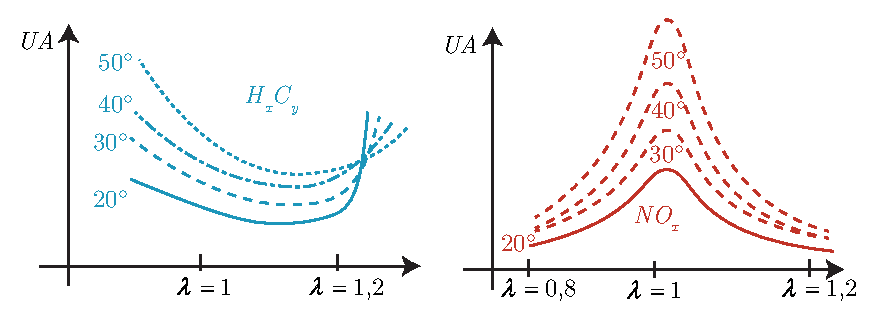
\includegraphics[width=.47\textwidth]{fig/aperturaEscapeGases.eps}
    \caption{Efecto de apertura de escape (AE) sobre los gases de escape producidos. La producción de $CO$ aumenta a mezclas más ricas ($\lambda<1$) con el aumento del AE.}
    \label{fig:aperturaEscape}
\end{figure}
\subsection[Sonda Lambda]{Sonda $\lambda$}
La sonda lambda mide la \textit{proporción} de $O_2$ presente en una mezcla de gases.
\[
\lambda = \frac{\textrm{Proporción de $O_2$ medida}}{\textrm{Proporción de $O_2$ teórica}}
\]

El valor $\lambda$ es la razón entre la proporción oxigeno presente en los gases de escape y la proporción de oxigeno teórica que debería estar presente después de una combustión estequiométrica.

{\color{magenta}La sonda $\lambda$ no mide el oxigeno de la mezcla antes de la combustión, está ubicada en el escape!} Cuando $\lambda =1$ se tiene una mezcla estereométrico, llamada la \emph{Zona Lambda}. Si $\lambda<1$ se dice que se tiene una mezcla rica (en combustible) y vice versa. 

Se suele trabajar con dos sondas cuando se quiere verificar el correcto funcionamiento del catalizador, la sonda lambda primaria (antes del catalizador) y la sonda lambda secundaria (después del catalizador). Comparando las lecturas de ambas se debería ver una disminución del oxigeno (porque hay oxidación ocurriendo en el catalizador!).

El motor puede trabajar en ``Lazo abierto'' o ``Lazo cerrado'' en conjunto con la Sonda Lambda. 

{\bf Lazo cerrado.} El motor busca reducir contaminación disminuyendo o aumentando tiempo de inyección según la lectura de la Sonda Lambda. En este régimen la señal oscila entre $100$mV y $900$mV,

{\bf Lazo abierto.} En ciertas situaciones no es posible trabajar con valores de mezcla estequiométricas. Si se tiene un motor en frío, o en aceleración brusca la central de control no ajusta la mezcla con valores estequiométricos, funcionamiento denominado \emph{lazo abierto}.

\begin{figure}[!htb]
    \centering
    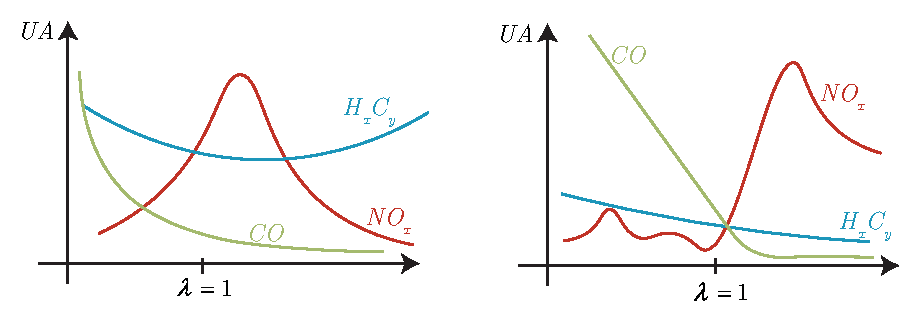
\includegraphics[width=.47\textwidth]{fig/lambdaEscape.eps}
    \caption{Medición sonda $\lambda$ antes y después del catalizador. La curva del $CO_2$ antes del catalizador es idéntica al \NX{} pero con el pico en $\lambda=1$}
    \label{fig:lambdaCatalizador}
\end{figure}

{\bf Catalizador}

Idealmente hace reaccionar todos los gases nocivos, efectivamente neutralizando la huella ambiental \emph{casi} por completo. 

Funciona a $400-700 ^\circ C$ con una mezcla del alrededor de $\lambda =1$ para lograr maximizar su efectividad. Se busca oxidar: $2CO+O_2\rightarrow 2CO_2$, $H_xC_y+(\frac{x}{4}+y) O_2\rightarrow \frac{x}{2} H_2O+y CO_2$ (reacciónes exotérmicas)  y reducir los óxidos del nitrógeno $2NO_x\rightarrow N_2+xO_2$. Se espera que a la salida del catalizador la lectura de la sonda lambda secundaria sea menor a la primaria
\subsection{Control de mezcla}
\begin{itemize}
    \item \textbf{Cut-off}. Cuando hay un cierre abrupto de la mariposa (se suelta el pedal de aceleración a RPM altas) se advierte al ECU. La ECU corta el suministro de combustible y fija el AE para evitar la formación de \HC
  
    \item \textbf{Ralentí}. Al número mínimo de revoluciones se inyecta pequeñas cantidades de combustible para permanecer en funcionamiento
    \item \textbf{Dash Pot} o \textbf{retardo de cierre de mariposa}. Impide el cierre total de la mariposa para prevenir la formación de \HC
\end{itemize}
\subsection{Válvula EGR}
Recirculación de gases de combustión que enfrían la cámara reduciendo así la cantidad de \NX producido. Disminuye la potencia, la eficacia del lubricante (introduce material particulado). La válvula EGR no actúa en ralentí, \NX, motor frío o baja carga.

{\bf Eliminación de gases de cárter de motor.}
$CO$ en bajas proporciones y \HC en altas proporciones. Originan de evaporación de compuestos de aceite y restos de combustible y gases de combustión que se escapan de la cámara a través de los aros del pistón. Conlleva con una \emph{perdida de potencia, aparición de incrustaciones en trayecto admisión--cámara}.

{\bf Vapores de tanque de combustible.} 
Se almacenan los vapores formados en el tanque adentro de un canister de carbón activado que son alimentados a la cámara por medio de una electroválvula.

{\bf Inyección de aire.}
Se puede inyectar aire al trayecto después de la válvula de escape para realizar una post-combustión del $CO$ y \HC para aliviar la tarea del catalizador.

{\bf Bomba de combustible.}
La bomba de combustible tiene el trabajo de presurizar el combustible para la inyección.

{\bf Regulador de presión de combustible.}
Se trata de mantener la diferencia de presión entre el combustible y el múltiple de admisión siempre igual. Estudiar las diferentes posiciones posibles del regulador (con retorno/sin retorno/demanda controlada)

{\bf Atenuador de pulsaciones.}
Amortigua pulsaciones en el fluido de la rampa de inyectores mediante un resorte.


\subsection{Actuadores}

{\bf Inyectores.}
Electrovalvulas 

{\bf Bomba lineal.}
La cantidad de elementos de bombeo es igual al número de cilindros en el motor y se situan en linea. 

Esta hecha de los siguientes elementos 

\begin{itemize}
    \item La bomba (generador de presión)
    \item El regulador mecánico (regula RPM según régimen)
    \item El variador de avance (ajusta el comienzo de inyección en función del número de revoluciones)
    \item Arbol de levas
\end{itemize}

Conocer bien la función de los reguladores mecánicos.

\subsection{Diesel bomba EDC}
Bomba aspira combustible, lo presuriza hasta la presión de inyección.

El combustible pasa a través de una bomba de transferencia rotativa que alimenta la cámara de compresión de émbolos radiales \emph{cuando la electroválvula se abre}.

Cuando la electroválvula se cierra, el combustible de la cámara de compresión se dirige al inyector correspondiente. Una vez que termina la inyección la electroválvula se abre y cae la presión nuevamente.

{\bf Avance de inyección.} 
Se realiza mediante la acción del embolo del corrector sobre el embolo de control

\subsection{Common Rail}
Controla la inyección de combustible Diesel en el momento correcto, con el caudal correcto y con la presión necesaria. Se reduce el ruido y favorece el motor.

Se compone de:
\begin{itemize}
    \item Unidad de control
\item Bomba de alta presión
\begin{itemize}
    \item Válvula de desconexión del elemento
    \item Válvula reguladora de presión
    \item Previo a la entrada de la bomba: Filtro de combustible y bomba previa
\end{itemize}
\item Acumulador de alta presión (Rail)
\begin{itemize}
    \item Sensor de presión Rail
\end{itemize}
\item Inyectores
\item Medidor de masa de aire
\item Sensor de revoluciones de cigüeñal
\item Sensor de temperatura del líquido refrigerante
\item Filtro de combustible
\item Sensor del pedal del acelerador
\item Turbocompresor
\end{itemize}

{\bf Diferencias con inyectores convencionales}
\begin{itemize}
    \item Presión constante después de un cierto número de vueltas (convencionales aumenta linealmente)
    \item Presión de inyección constante durante inyección. Las combustiones favorables requieren pequeños caudales al comienzo de la inyección. Por eso el sistema Common Rail cuenta con una inyección previa pequeña ($1-4\si{mm^2}$)
\end{itemize}

{\bf Características de la inyección previa.}
Puede estar adelantada del PMS hasta $90^\circ$ aunque antes de los $40^\circ$ esto puede ocasionar problemas al tener contacto entre el combustible y las paredes del cilindro y pistón, provocando una dilución inadmisible del aceite lubricante.

Con la inyección previa se logra que \emph{la presión de compresión aumente ligeramente mediante una combustión parcial previa al PMS, reducir el retardo de encendido a la inyección principal, reducir el aumento de la presión de combustión y suavizar los picos de presión.}

{\bf Características de la inyección posterior.}
Se puede aplicar por los efectos reductores de los aditivos del combustible. Puede suceder hasta $200^\circ$ después del cigüeñal durante la etapa de expansión o escape.

\subsection{Combustible}
{\bf Reacciones.}
Recordemos que el aire es una mezcla de varios gases. En su mayor parte es Nitrogeno (78,09\%), oxigeno (20,95\%) y argon (0,93\%). $\frac{78,09}{20,95}=3,73$  
La reacción general para aire en exceso:
\begin{align*}
C_m H_n O_p+Y O_2+&3,73Y(N_2)\longrightarrow \\ mCO_2 +\tfrac{n}{2}& H_2O +3,73 Y (N_2)+(Y-Y_{cc})O_2
\end{align*}
donde $Y$ es la cantidad de moles de oxigeno suministrados. $Y_{cc}$ es la cantidad de moles de oxigeno requeridos para lograr la reacción estequiométrica.

En el caso que $Y=Y_{cc}$ entonces se tiene una mezcla estequiometrica y no se produce $O_2$.

La reacción general para mezcla rica:
\begin{align*}
C_mH_nO_p+&YO_2+3,73YN_2\longrightarrow \\ &XCO+(m-X)CO_2+\tfrac{n}{2}H_2O+3,73YN_2
\end{align*}
\begin{align*}
\frac{p}{2}+Y=\frac{X}{2}+&(m-X)+\frac{n}{4}\\
&\Rightarrow X=2\left(m+\frac{n}{4}-\frac{p}{2}-Y \right)=2(Y_{cc}-Y)
\end{align*}
la formula queda 

\begin{align*}
C_mH_nO_p + YO_2+3&,73YN_2\longrightarrow \\  2(Y_{cc}-Y)CO+2(&Y -Y_{min})CO_2+\tfrac{n}{2}H_2O+3,73YN_2
\end{align*}

{\bf Hidrocarburos liquidos.}
\begin{itemize}
\item Bencinas o Gasolina=nafta. Motores encendidos por chispa.
\item Gasóleos: Gasoil, fuel oil etc.
\item Kerosene. Alto poder calorifico. No se suele usar por su alta viscosidad y contaminación.
\item Benzol y alcoholes. Considerados carburantes
\end{itemize}

{\bf Poder antidetonante o número de octano (NO).}
Se obtiene comparando el carburante con combustibles de referencia: el \emph{iso-octano} y el \emph{heptano}\footnote{Antiguamente iso-octano y tetraetil de plomo.}
Iso-octano tiene cualidades muy antidetonantes y se lo toma como referencia $NO=100$. El Heptano en cambio detona con facilidad $NO=0$.

Un combustible que a la misma relación de compresión que una mezcla 80\% de iso-octano y 20\% heptano, tiene un $NO=80$.

{\bf Formas de medir el} $NO$.
\begin{itemize}
    \item $RON$ Research Octane Number: Asociado al funcionamiento con altas velocidades y detonación media o suave
    \item $MON$ Motor Octane Number: Asociado a velocidades altas, temperaturas y funcionamiento a media o alta carga.
\end{itemize}

\section{Lubricantes}
Tres tipos básicos de lubricación. Hidrodinámico o fluido, rozamiento semifluido, rozamiento seco. Lo ideal es llegar a lubricar hidrodinámico (no hay contacto entre partes solidas).

{\bf Funciones y algunas propiedades necesarias del aceite lubricante:}%iento lo máximo posible ento lo máximo posible
\begin{itemize}
\item Refrigerar zonas a lubricar. Refrigerar zona interior del pistón.
\item Aumentar estanqueidad entre segmentos y el cilindro elevando la compresión
\item Amortigua las cargas fluctuantes sobre cojinetes
\item Limpia y transporta carbonilla y partículas al filtro.
\item \textbf{Protege contra la corrosión.} Previene formación de ácidos que carcomen la parte más frágil del motor: bujes de apoyo del cigüeñal y árbol de levas.
\item Se lo aditiva así mantiene la viscosidad en caliente y la fluidez en frío. Hoy en día TODOS los aceites tienen aditivos.
\begin{itemize}
    \item \textbf{Detergente.} Limpia partes mecanicas
    \item \textbf{Dispersante.} ``Rodea" particulas sueltas y evita formación de compuestos
    \item \textbf{Antiespumante.} Evita formación de burbujas para no disminuir capacidad lubricante
\end{itemize}
\item El aceite que pasa a la cámara tiene que quemarse sin dejar residuos
\item Untuoso: Capacidad de adherirse a las superficies metálicas
\item 
\end{itemize}

\subsection{Parámetros característicos de un lubricante.}
Las escalas de SAE se usan para medir la viscosidad de un aceite.
{\bf Índice de viscosidad.}
El \emph{viscosity index} o $VI$ nos dice cuanto varía la viscosidad ante un cambio de temperatura.
\[
\frac{\di \mu}{\di T}\propto VI^{-1}
\]
osea que la viscosidad de un lubricante con alto $VI$ no varía fuertemente con cambios de temperatura.

Un aceite \textbf{multigrado}, a diferencia de un aceite monogrado tiene mayor margen de temperatura de trabajo (alto $VI$). Esto se logra con aditivos. SAE los denomina con una ``W". Un \textit{SAE 20W 40} se comporta como un \textit{SAE 20} a bajas temperaturas y como un \textit{SAE 40} a altas temperaturas.

{\bf Total Base Number (TBN).}
La propiedad \textit{detergente} de los aceites. Gracias a esta propiedad los aceites mantienen en suspensión las partículas, evitando que entren en contacto con superficies e incrustaciones.

Los aditivos que logran esta mejora (\textbf{TBN}) son químicamente \textit{básicos}. De está forma contrarrestan también la formación de ácido sulfúrico ($H_2SO_4$) por causa del contenido de azufre en el combustible. Suele pasar con Diesel por el alto contenido de azufre.

{\bf Clasificación API.}
Usada en EE.UU y la mayor parte de latinoamerica.\footnote{En europa el organismo de control es la ACEA}. Las categorías API se dividen en dos series:
\begin{itemize}
\item S - Spark ignition (motores Otto)
\item C - Compression (motores Diesel)
\end{itemize}
El número que procede a las letras de categoría es el tiempo del motor (dos tiempos/cuatro tiempos).
 
Si se indica que es ``Plus'' es porque cumple con las especificaciones de la categoría indicada y los \textit{excede!} Esto no significa que cumple con las especificaciones de la próxima categoría!

\textbf{El API Doughnut}
Un ejemplo de una clasificación API: \texttt{API SERVICE CI-4/SL} Nos dice que es un aceite para motores Diesel de \textbf{4} tiempos con la posibilidad de usarse con motores de Otto calificados para \textbf{SL}. (C=Compression Ignition, S=Spark Ignition). La clasificación del aceite es \textbf{SL}, una clasificación anterior a  \textbf{SN} aún no obsoleta.
\begin{figure}[htb!]
    \centering
    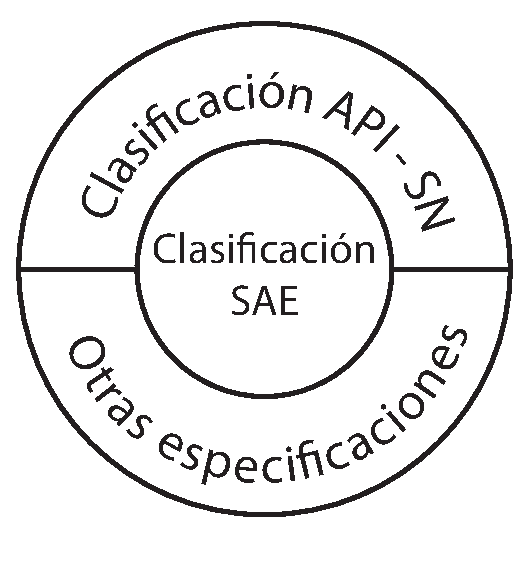
\includegraphics[width=.25\textwidth]{fig/api.eps}
    \caption{Como ubicarse con un API ``doughnut". Las últimas letras son \emph{SN}, la clasificación del aceite, en este caso para motor Otto. En el momento que fue escrito este documento la última clasificación del API era la SN Plus para motores Otto aprobada el 9 de noviembre 2017 y CK-4 para motores Diesel aprobada 2017. Existe la clasificación FA-4 para motores Diesel de bajo contenido de sulfuro ($<$0,0015\%), introducida 2017.}
    \label{fig:APIclasification}
\end{figure}

\subsection{Sistema de lubricación del motor endotérmico}
\begin{itemize}
    \item Engrase a presión (el más utilizado). Típica presión de engrase: 0,5-1 bar a ralentí. 3-5 bar en régimen
    \item Engrase por mezcla con el combustible
\end{itemize}

{\bf Engrase a presión.} El aceite pasa por los canales del block y la culata, lubrica los cojinetes, rebalsa y cae al cárter. En el cárter es succionado por la bomba haciéndolo pasar por un filtro y al conducto principal y se repite. A la salida de la bomba hay una válvula de descarga que limita la presión máxima del aceite.

Los apoyosLos componentes engrasados a presión 

\textbf{Filtro.} Cuando está puesto en \textit{serie} todo el aceite pasa por el filtro. Menos común son los filtros de \textit{derivación} que solo filtran el aceite del cárter. Como regla general se suele cambiar el filtro cada 15000 km o al año.